%%%%%%%%%%%%%%%%%%%%%%%%%%%%%%%%%%%%%%%%%%%%%%
%Lab report writeup based on template by Derek Hildreth
%%%%%%%%%%%%%%%%%%%%%%%%%%%%%%%%%%%%%%%%%%%%%%

%\documentclass[aps,letterpape,10pt]{revtex4}
\documentclass[aps,letterpaper,10pt]{article}
%\documentclass{article}

\usepackage{graphicx} % For images
\usepackage{float}    % For tables and other floats
\usepackage{verbatim} % For comments and other
\usepackage{amsmath}  % For math
\usepackage{amssymb}  % For more math
\usepackage{fullpage} % Set margins and place page numbers at bottom center
\usepackage{subfig}   % For subfigures
\usepackage[usenames,dvipsnames]{color} % For colors and names
\usepackage{fancyhdr} %headers
\usepackage{listings} %for code
\usepackage{color} %to color code
\usepackage{wrapfig} % for inline images

%Color and code setup
\definecolor{dkgreen}{rgb}{0,0.6,0}
\definecolor{gray}{rgb}{0.5,0.5,0.5}
\definecolor{mauve}{rgb}{0.58,0,0.82}
\definecolor{codebg}{rgb}{.95,.95,.98}

\lstset{ %
	language=Java,
	tabsize=4, 
	numbers=left,
	numberstyle=\footnotesize,
	backgroundcolor=\color{codebg},
	breaklines=true,
	breakatwhitespace=true,
	basicstyle=\small,
	numberstyle=\tiny\color{black},
	showstringspaces=false,
	keywordstyle=\color{blue}, 
	stringstyle=\color{dkgreen},
	commentstyle=\color{gray},
	frame=single,
	title = \texttt{\lstname}
	}

%%%%%%%%%%%%

%HEADER FORMATING%%%%%%%%%%%%%
\pagestyle{fancy}
\headheight 23pt
\setlength{\headsep}{20pt}
\lhead{PHYS 251 - Prof. Tom Witten \\ Problem 6.5}
\rhead{A. Athanassiadis\\Due 11/19/2012}
%%%%%%%%%%%%%%%%%%%%%%%%

%Custom Definitions%%%%%%%%%%%%%%%
\newcommand{\ttt}{\texttt}
%%%%%%%%%%%%%%%%%%%%%%%%

\begin{document}

\section{Problem 6.5: Behavior of Runge-Kutta Solutions}
\subsection*{a}
\begin{center}
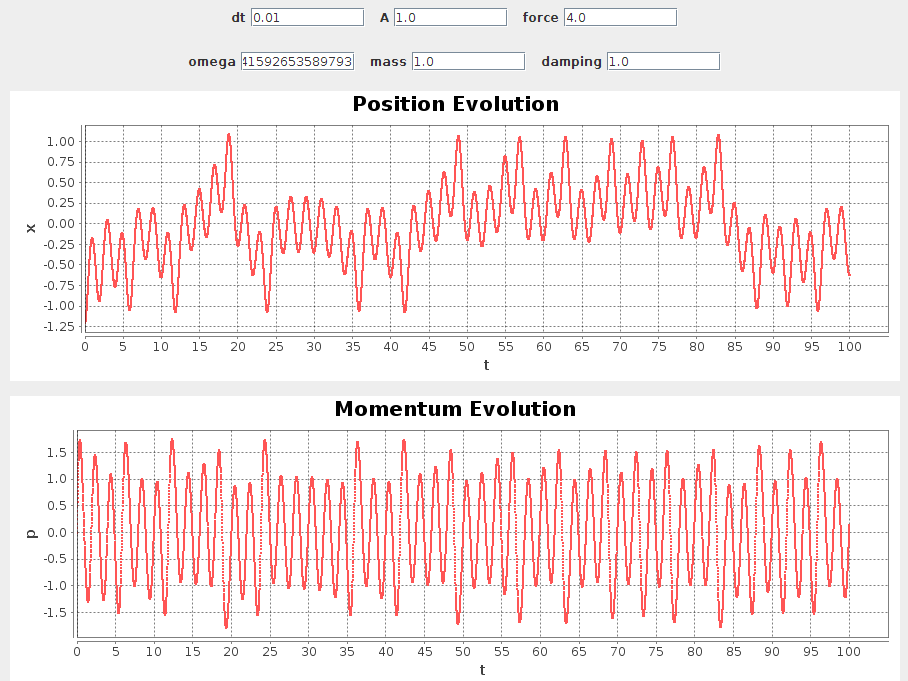
\includegraphics[width=.6\textwidth]{../img/ChaoticInitial.png}
\end{center}

When using the default parameters, there is very little apparent periodicity in $x$ and $p$. By eye, it looks as though there could be some high-frequency periodicity that further analysis could separate (fourier decomp). However, this is just speculative. There is no clear periodic trend, and the motion seems chaotic.

\newpage
\subsection*{b}
\begin{center}
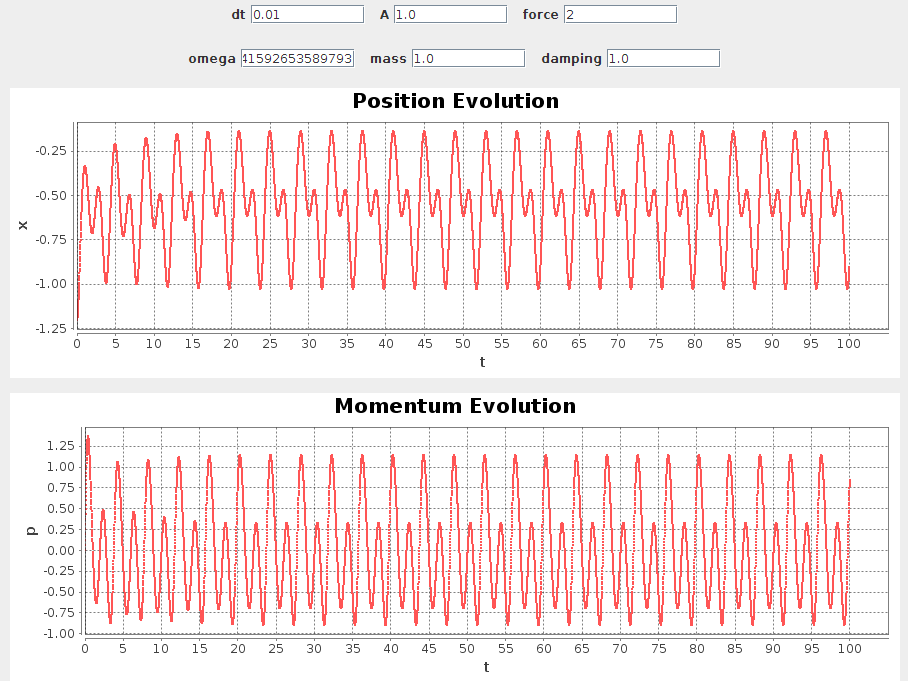
\includegraphics[width=.6\textwidth]{../img/Initialby2.png}
\end{center}
As the driving force amplitude is reduced, the time evolution of $x$ and $p$ begin to look periodic. For $|F| = F_0/2$, the periodicity seems like a complex superposition of two different functions.

\begin{center}
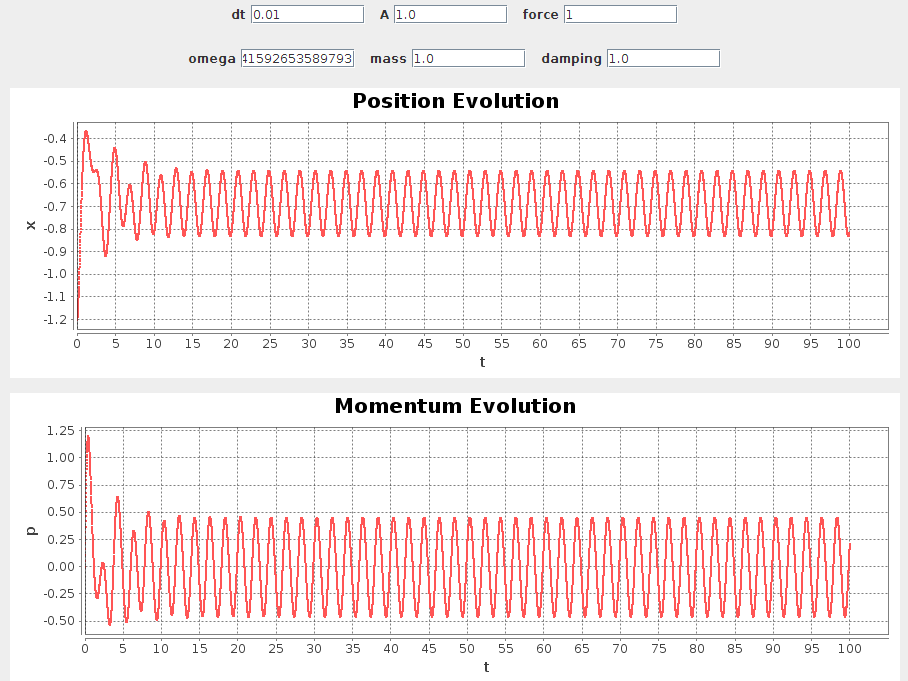
\includegraphics[width=.6\textwidth]{../img/Initialby4.png}
\end{center}
As the driving amplitude is reduced further ($|F| = F_0/4$), the time evolution of $x$ and $p$ rapidly converge to simple periodic oscillations with a frequency of motion equal to the driving frequency. The picture below shows this same behavior zoomed in on the $x$ vs $t$ plot. Clearly, the period of oscillation is $T = 2$. Comparing with the driving frequency, we see that $T_d = 2\pi / \omega = 2\pi/\pi = 2$. Thus the system is moving at the driving frequency.

\begin{center}
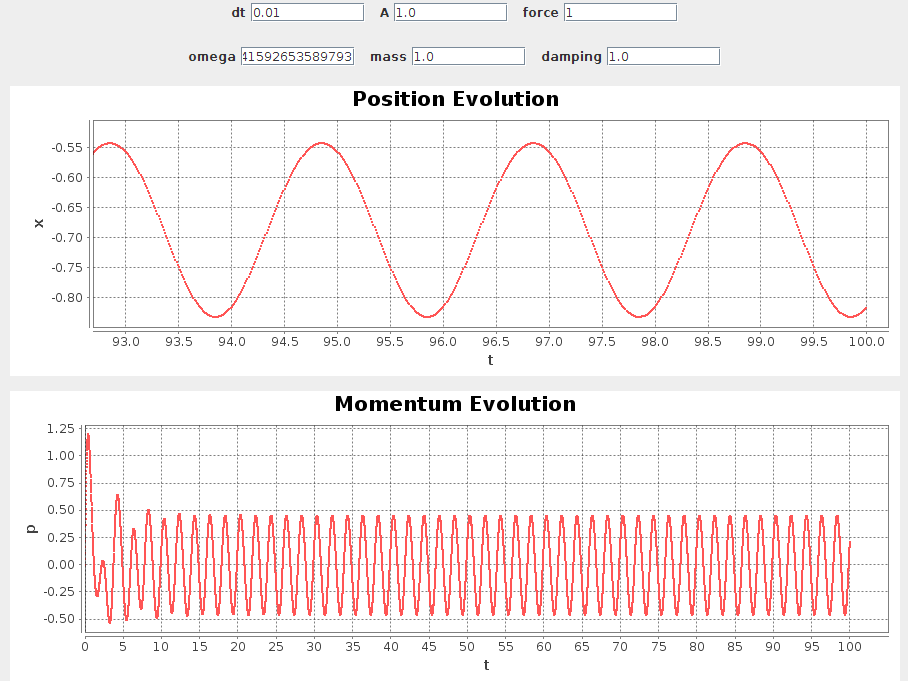
\includegraphics[width=.6\textwidth]{../img/Initialby4Zoom.png}
\end{center}

\newpage
\subsection*{c}
\begin{center}
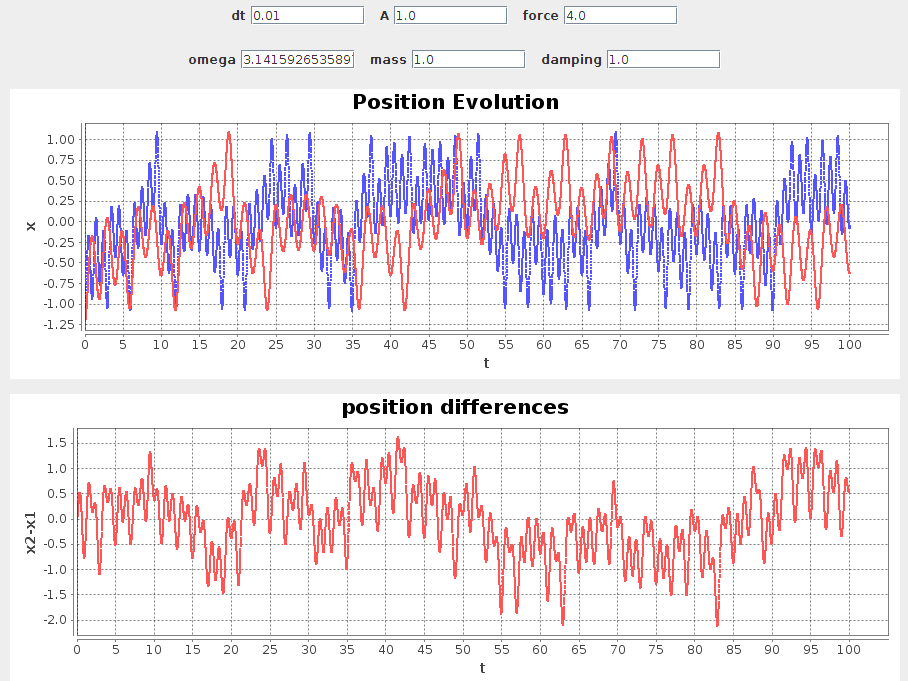
\includegraphics[width=.6\textwidth]{../img/dw2-1.png}
\end{center}

To estimate the error from the numerical solving, I compared the results of the original calculations to those attained by the same system, but with half the time resolution. The two runs are plotted in red (original) and blue (half resolution) above. As the plots indicate, for approx. the first 50 time-steps (counting with the original resolution), the two produce the same results. However, they then begin to deviate from one another and follow completely different paths. Note that since one was stepping twice as fast as the other, it was only polled half as often so that the two could be properly compared as $x_2(t) - x_1(t)$.

\newpage
\subsection*{d}
\begin{center}
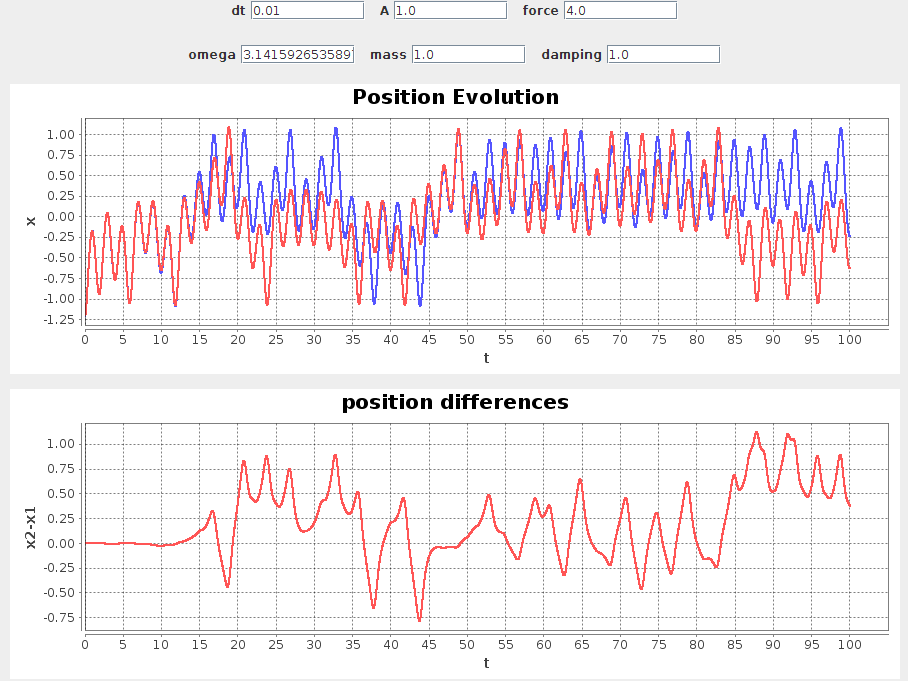
\includegraphics[width=.6\textwidth]{../img/dw2-2.png}
\end{center}

I checked error similarly using a perturbation in the initial condition. The original (blue) and the offset ($x_{0,2}$ = 1.001 * $x_{0,1}$, red) plots are given above as well as their differences. Note that this time, they diverge from each other after only $\approx15$ time steps (this time they have the same dt).

For the system to be characterizable by a Lyapunov exponent, the small perturbation to $x(0)$ should have caused exponential divergence in $x(t)$. Looking up to $t\approx 17$, this looks rather feasible. The difference $x_2 - x_1$ seems to grow exponentially. To estimate the Lyapunov exponent, $\lambda$, I can look at how long in time it takes $x(t)$ to decline by a factor of $e$. Using $x(17)\approx .33$ and $e\approx 3$, I can estimate this to be $dt \approx .5$. Thus the Lyapunov exponent is approximately $\lambda = 2$.

$\lambda$ is clearly positive in the plot. This indicates that the double oscillator dynamics are chaotic, since small initial perturbations lead to exponentially diverging states.

\end{document} 
